\documentclass[journal,12pt,twocolumn]{IEEEtran}
%
\usepackage{setspace}
\usepackage{gensymb}
\usepackage{xcolor}
\usepackage{caption}
%\usepackage{subcaption}
%\doublespacing
\singlespacing
\usepackage{multicol}
%\usepackage{eenrc}
\usepackage{iithtlc}
%\usepackage{graphicx}
%\usepackage{amssymb}
%\usepackage{relsize}
\usepackage[cmex10]{amsmath}
\usepackage{mathtools}
%\usepackage{amsthm}
%\interdisplaylinepenalty=2500
%\savesymbol{iint}
%\usepackage{txfonts}
%\restoresymbol{TXF}{iint}
%\usepackage{wasysym}
\usepackage{amsthm}
\usepackage{mathrsfs}
\usepackage{txfonts}
\usepackage{stfloats}
\usepackage{cite}
\usepackage{cases}
\usepackage{subfig}
%\usepackage{xtab}
\usepackage{longtable}
\usepackage{multirow}
%\usepackage{algorithm}
%\usepackage{algpseudocode}
\usepackage{enumitem}
\usepackage{mathtools}
%\usepackage{stmaryrd}
\usepackage{graphicx}
\usepackage{listings}
    \usepackage[latin1]{inputenc}                                 %%
    \usepackage{color}                                            %%
    \usepackage{array}                                            %%
    \usepackage{longtable}                                        %%
    \usepackage{calc}                                             %%
    \usepackage{multirow}                                         %%
    \usepackage{hhline}                                           %%
    \usepackage{ifthen}                                           %%
  %optionally (for landscape tables embedded in another document): %%
    \usepackage{lscape}     
\usepackage{url}
\def\UrlBreaks{\do\/\do-}

%\usepackage{wasysym}
%\newcounter{MYtempeqncnt}
\DeclareMathOperator*{\Res}{Res}
%\renewcommand{\baselinestretch}{2}
\renewcommand\thesection{\arabic{section}}
\renewcommand\thesubsection{\thesection.\arabic{subsection}}
\renewcommand\thesubsubsection{\thesubsection.\arabic{subsubsection}}

\renewcommand\thesectiondis{\arabic{section}}
\renewcommand\thesubsectiondis{\thesectiondis.\arabic{subsection}}
\renewcommand\thesubsubsectiondis{\thesubsectiondis.\arabic{subsubsection}}

% correct bad hyphenation here
\hyphenation{op-tical net-works semi-conduc-tor}

\def\inputGnumericTable{}  

\lstset{
language=python,
frame=single, 
breaklines=true
}

\begin{document}
%

\theoremstyle{definition}

\newtheorem{theorem}{Theorem}[section]
\newtheorem{problem}{Problem}
\newtheorem{proposition}{Proposition}[section]
\newtheorem{lemma}{Lemma}[section]
\newtheorem{corollary}[theorem]{Corollary}
\newtheorem{example}{Example}[section]
\newtheorem{definition}{Definition}[section]
%\newtheorem{algorithm}{Algorithm}[section]
%\newtheorem{cor}{Corollary}
\newcommand{\BEQA}{\begin{eqnarray}}
\newcommand{\EEQA}{\end{eqnarray}}
\newcommand{\define}{\stackrel{\triangle}{=}}

\bibliographystyle{IEEEtran}
%\bibliographystyle{ieeetr}



\providecommand{\pr}[1]{\ensuremath{\Pr\left(#1\right)}}
\providecommand{\qfunc}[1]{\ensuremath{Q\left(#1\right)}}
\providecommand{\sbrak}[1]{\ensuremath{{}\left[#1\right]}}
\providecommand{\lsbrak}[1]{\ensuremath{{}\left[#1\right.}}
\providecommand{\rsbrak}[1]{\ensuremath{{}\left.#1\right]}}
\providecommand{\brak}[1]{\ensuremath{\left(#1\right)}}
\providecommand{\lbrak}[1]{\ensuremath{\left(#1\right.}}
\providecommand{\rbrak}[1]{\ensuremath{\left.#1\right)}}
\providecommand{\cbrak}[1]{\ensuremath{\left\{#1\right\}}}
\providecommand{\lcbrak}[1]{\ensuremath{\left\{#1\right.}}
\providecommand{\rcbrak}[1]{\ensuremath{\left.#1\right\}}}
\theoremstyle{remark}
\newtheorem{rem}{Remark}
\newcommand{\sgn}{\mathop{\mathrm{sgn}}}
\providecommand{\abs}[1]{\left\vert#1\right\vert}
\providecommand{\res}[1]{\Res\displaylimits_{#1}} 
\providecommand{\norm}[1]{\lVert#1\rVert}
\providecommand{\mtx}[1]{\mathbf{#1}}
\providecommand{\mean}[1]{E\left[ #1 \right]}
\providecommand{\fourier}{\overset{\mathcal{F}}{ \rightleftharpoons}}
%\providecommand{\hilbert}{\overset{\mathcal{H}}{ \rightleftharpoons}}
\providecommand{\system}{\overset{\mathcal{H}}{ \longleftrightarrow}}
\providecommand{\gauss}[2]{\mathcal{N}\ensuremath{\left(#1,#2\right)}}
	%\newcommand{\solution}[2]{\textbf{Solution:}{#1}}
\newcommand{\solution}{\noindent \textbf{Solution: }}
\providecommand{\dec}[2]{\ensuremath{\overset{#1}{\underset{#2}{\gtrless}}}}
%\numberwithin{equation}{section}
%\numberwithin{problem}{section}

\def\putbox#1#2#3{\makebox[0in][l]{\makebox[#1][l]{}\raisebox{\baselineskip}[0in][0in]{\raisebox{#2}[0in][0in]{#3}}}}
     \def\rightbox#1{\makebox[0in][r]{#1}}
     \def\centbox#1{\makebox[0in]{#1}}
     \def\topbox#1{\raisebox{-\baselineskip}[0in][0in]{#1}}
     \def\midbox#1{\raisebox{-0.5\baselineskip}[0in][0in]{#1}}


% paper title
% can use linebreaks \\ within to get better formatting as desired

%\title{FM Signal Transmission Using Pi}
 
\title{
\logo{
FM Signal Transmission Using Pi
}
} 
 
%
%
% author names and IEEE memberships
% note positions of commas and nonbreaking spaces ( ~ ) LaTeX will not break
% a structure at a ~ so this keeps an author's name from being broken across
% two lines.
% use \thanks{} to gain access to the first footnote area
% a separate \thanks must be used for each paragraph as LaTeX2e's \thanks
% was not built to handle multiple paragraphs
%

%\author{Y Aditya, A Rathnakar and G V V Sharma$^{*}$% <-this % stops a space
\author{K Prasanna Kumar and G V V Sharma %<-this  stops a space
\thanks{The authors are with the Department
of Electrical Engineering, IIT, Hyderabad
502285 India $1^{st}$ e-mail: kk.prassu924@gmail.com, $2^{st}$e-mail: \{gadepall\}@iith.ac.in. 
}}



% make the title area
\maketitle


\tableofcontents

\bigskip

\begin{abstract}
This manual explains how to transmit the signals from Raspberry Pi using Frequency Modulation (FM). We use Raspberry Pi as FM transmitter \&  a copper wire connected to GPIO pin of Pi as antenna.  
\end{abstract}

\section{Download \& Install}

If you do not GIT installed use the following command.
\begin{lstlisting}[frame = single]
 sudo apt-get install git-core
\end{lstlisting}
Use the following commands to download FM transmitter code in raspberry pi.
\begin{lstlisting}{frame = single}
sudo apt-get update
git clone https://github.com/markondej/fm_transmitter
\end{lstlisting}
The clone or downloaded directory will be with name \textit{fm \_ transmitter}. So, rename the directory by using following command for future understanding
\begin{lstlisting}
mv fm_transmitter pifm
\end{lstlisting} 
Now compile the FM transmitter code (install FM transmitter software)
\begin{lstlisting}
sudo apt-get install make gcc g++
\end{lstlisting}
Use the above command to install 'make gcc g++'. If they already exists, then go to the directory \textit{pifm} and install or compile make file by using following commands
\begin{lstlisting}
cd pifm
make
\end{lstlisting}
Now FM transmitter (code) is installed in Pi, we can see a file "fm \_ transmitter" in the  \textit{pifm} directory. To check that type
\begin{lstlisting}
ls
\end{lstlisting} 

\section{Hardware Setup}
External hardware required to build an FM transmitter using Pi is a female to male jumper wire. Connect jumper wire to the pin number 7 of Pi, since it is an output pin for FM signal \& the pin with wire acts as an FM antenna.   
\begin{center}
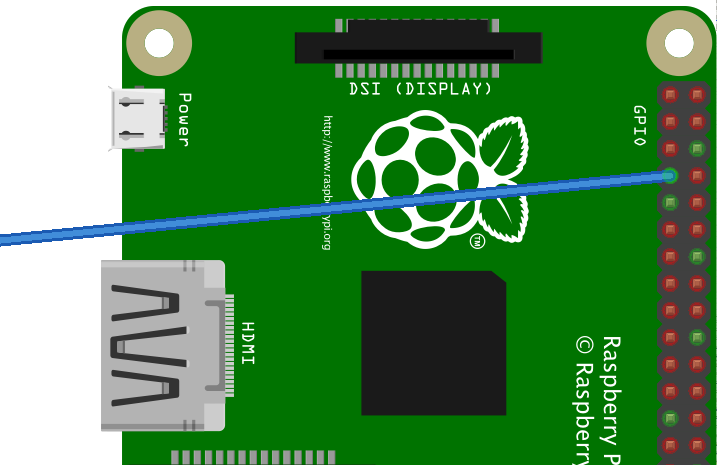
\includegraphics[scale=0.2]{Figures/pifm}
\end{center}
\section{Working}
Run the following commands to transmit FM signals using Pi  
\begin{lstlisting}
cd 
cd pifm
sudo ./fm_transmitter -f [frequency] -r [filename]
\end{lstlisting}
In the above command [frequency] means the transmitting frequency, enter any value in between 87 to 108. Enter the name of the file or directory of the .wave file in [filename]. For example
\begin{lstlisting}
sudo ./fm_transmitter -f 89.9 -r sound.wave
\end{lstlisting}
\begin{center}
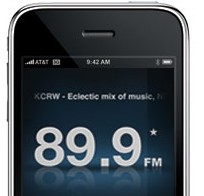
\includegraphics[scale=0.5]{Figures/iphone_radio}
\end{center}


\textbf{Note:-} It can transmit only .wave file not mp3 or mpeg file. So, the file which we want to transmit should be converted to .wave\\

Transmit audio from USB sound card connected to the pi by using following command

\begin{lstlisting}
  arecord -D plughw:1,0 -c1 -d 0 -r 22050 -f S16_LE | sudo ./fm_transmitter -f 100.6 -
\end{lstlisting}


%\begin{thebibliography}{00}
%\bibitem{b1}Wiring Pi- GPIO Interface library for the Raspberry Pi, url{http://www.wiringpi.com/}. 
%\bibitem{b2} Sunfounder, Raspberry pi tutorial - 'Lesson 2 Controlling an LED by a Button' \url{https://www.sunfounder.com/}. Demo video link \url{https://www.youtube.com/watch?time_continue=4&v=y3Pv7--6eik}.
%\end{thebibliography}
\end{document}